%----------------------------------------------------------------------------------------
%	Inställningar och dokumentkonfiguration
%----------------------------------------------------------------------------------------

\documentclass[paper=a4, fontsize=11pt]{report} % A4-sida och 11 punkters fontstorlek

\usepackage[T1]{fontenc} % 8-bitarskodning som har 256 glyfer
\usepackage[english]{babel} % Svenskt språk
\usepackage[utf8]{inputenc} % För svenska tecken
\usepackage{dtklogos} % Logos
\usepackage{wallpaper} % Bakgrundsbild
\usepackage{fancyhdr} % Specialsidhuvud och sidfot
\usepackage{enumerate} 
\usepackage{xifthen}% provides \isempty test
\usepackage{listings}% Code examples
\usepackage{xcolor}
\newcounter{tmpc}
\lstdefinestyle{BashInputStyle}{
  language=bash,
  basicstyle=\footnotesize\ttfamily,
  numbers=left,
  numberstyle=\tiny,
  numbersep=3pt,
  frame=tb,
  columns=fullflexible,
  backgroundcolor=\color{yellow!20},
  linewidth=0.9\linewidth,
  xleftmargin=0.1\linewidth
}
% Exampels
% Inline
% \lstinline[style=BashInputStyle]´# apt-get --purge remove rubygems´.
% Multiline
% \begin{lstlisting}[style=BashInputStyle]
%    # apt-get --purge remove rubygems
% \end{lstlisting}

\pagestyle{fancyplain} % Använd sidhuvud och sidfot på alla sidor
\fancyhead[L]{Seminar 3 -- 1DV020 -- 2015 -- Server Administration} % Titel till vänster i sidhuvud
\fancyhead[C]{} % Tomt i mitten
\fancyhead[R]{} % Tomt till höger
\fancyfoot[L]{} % Tomt till vänster
\fancyfoot[C]{} % Tomt i mitten
\fancyfoot[R]{\thepage} % Sidnumrering till höger i sidfoten
\renewcommand\thesection{\arabic{section}} % Section beter sig som i dokumentklassen article

\newcommand{\win}[1]{Microsoft Windows Server\ifthenelse{\isempty{#1}}{}{ #1}}
\newcommand{\gui}[0]{``Server with a GUI''}
\newcommand{\core}[0]{Windows Server Core}
%----------------------------------------------------------------------------------------
%	TITLE SECTION
%----------------------------------------------------------------------------------------
\newcommand\BackgroundPic{
    \put(-50,-50){
    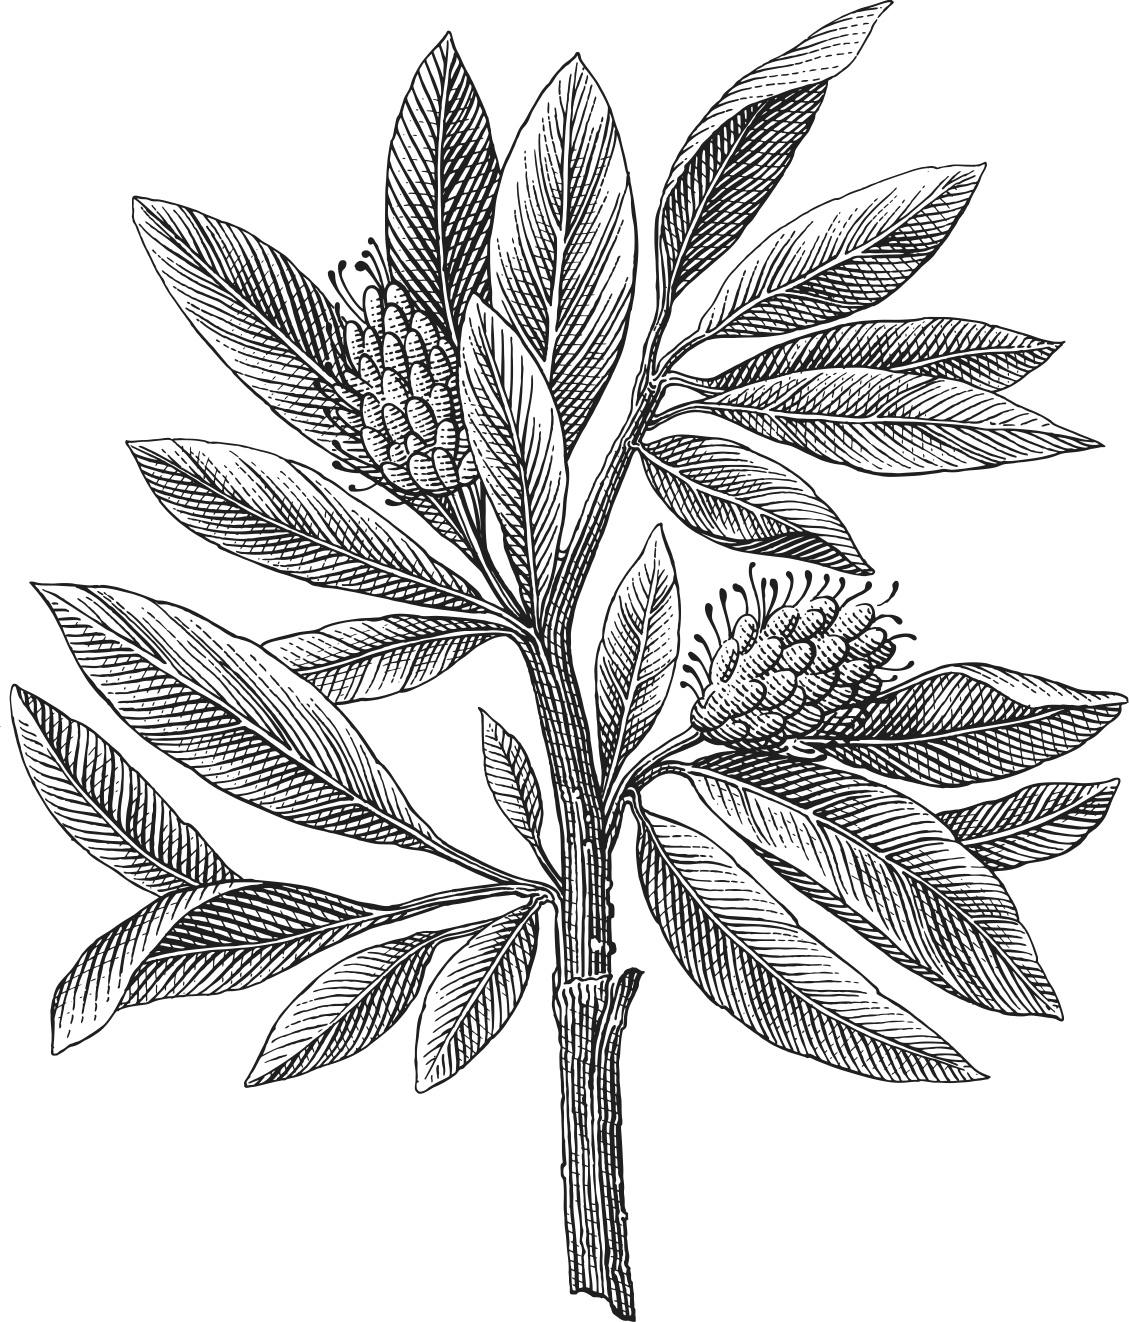
\includegraphics[keepaspectratio,scale=0.65]{lnu_etch.png} % Bakgrundsbild
    }
}
\newcommand\BackgroundPicLogo{
    \put(15,700){
    
\includegraphics[keepaspectratio,scale=0.10]{logo.png} % Logga i vänstra hörnet
    }
}

\newcommand{\horrule}[1]{\rule{\linewidth}{#1}} % Skapa hortisontell linje

\title{	\vspace{-10cm}
    \normalfont \normalsize
    \textsc{Linnaeus University} \\ [25pt] % Universitetes namn
    \horrule{0.5pt} \\[0.4cm] % Tunn linje högst upp
    \huge Seminar 2\\ % Arbetes titel
	\large \textcolor{gray}{1DV020 -- Server Administration}
    \horrule{0.5pt} \\[0.4cm] % Tunn linje längst ner
}

\author{Jacob Lindehoff} % Författarnas namn

\date{\normalsize\today} % Dagens datum

\begin{document}
  \AddToShipoutPicture*{\BackgroundPic} % Lägger in backgrundsbild på första sidan
  \AddToShipoutPicture*{\BackgroundPicLogo}
  \maketitle % Skriv ut titeln
  \noindent % Tabba inte in på första meningen

  %------------------------------------------------
  % Introduktion
  %------------------------------------------------
  \section{Introduction}
  During this seminar, we will address the following topics:
  \begin{itemize}
    \item DNS
    \item DHCP
    \item Web Server
  \end{itemize}

  %------------------------------------------------
  %	Deadline
  %------------------------------------------------
  \section{Deadline}
  The seminar is on the {\color{red}25th of February 2015} and it is compulsory. If you cannot participate, it must be notified in advance and a written report of the seminar must be submitted no later than {\color{red}3 days} after the seminar. The written report should contain detailed answers to all questions in the seminar.
  \newpage

  %------------------------------------------------
  %	Seminariefrågor
  %------------------------------------------------
  \section{Seminar Questions}
  \subsection{DNS}
  \begin{enumerate}
    \begin{large}
		\item What is DNS and its main function?
		\item What is Forward Lookup Zone?
		\item What is Reverse Lookup Zone?
		\item Please describe 10 different TLDs and its uses.
		\item Without DNS, the Internet would not work:
		\begin{enumerate}[a.]
			\item How does DNS structure on the Internet work?
			\item Must the company's DNS servers to be connected to the Internet's DNS servers?
			\item What is the difference between an internal DNS server from an public?
		\end{enumerate}
		\item How does a DNS delegation work and when is it used?
		\item How do you go about creating redundancy in a zone / domain?
		\item Describe the following records:
		\begin{enumerate}[a.]
			\item CNAME
			\item PTR
			\item MX
			\item SRV
			\item NS
			\item SOA
			\item A
		\end{enumerate}
		\item What is a Zone transfer?
		\item How dose ROOT hints work?
		\item Describe the advantages and disadvantages of DNS caching.
		\item What is DNS forward and how it works?
		\begin{figure}[h]
		\centering
		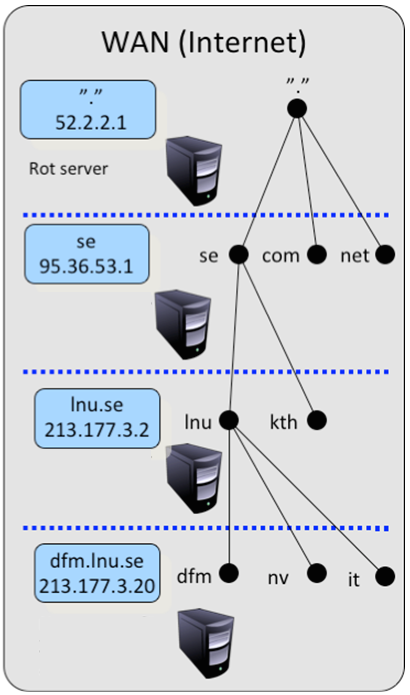
\includegraphics[width=0.5\linewidth]{./figure_1}
		\caption{Namne servers on the Internet}
		\label{fig:figure_1}
		\end{figure}
		
		\item Let's say you have a client that is connecting to a network that has its own DNS server that is configured with DNS forward to the company's ISP's DNS server. Start from Figure \ref{fig:figure_1}
		\begin{enumerate}[a.]
			\item Describe in detail what happens when the client makes a recursive DNS request for IP of www.dfm.lnu.se 
			\item Describe in detail what happens when the client makes a none recursive DNS request for IP of www.dfm.lnu.se 
		\end{enumerate}
    \end{large}
    \setcounter{tmpc}{\theenumi}
  \end{enumerate}

  \subsection{DHCP}
  \begin{enumerate}
  \setcounter{enumi}{\thetmpc}	
    \begin{large}
	    \item What is DHCP and how this simplifies administration?
		\item Describe the following DHCP terms:
		\begin{enumerate}[a.]
			\item Scope
			\item Exclusion range
			\item Address pool
			\item Lease
			\item Reservation
		\end{enumerate}
		\item Describe the different steps of a DHCP request?
    \end{large}
    
    \setcounter{tmpc}{\theenumi}
  \end{enumerate}
  \newpage
  \subsection{Web server}
  \begin{enumerate}
  \setcounter{enumi}{\thetmpc}
    \begin{large}
    	\item Question
    \end{large}
  \end{enumerate}
\end{document}
